\subsubsection{Sourcing Current}
For this second iteration the low power of the shelf linear regulator has been replaced with a custom discrete 12 A adjustable linear regulator based on the LT3080-1 from Linear Technologies.

The first thoughts were to make a fully discrete solution but since the low permitted forward voltage drop of the regulator combined with the big output current of 12 A and relatively big range (of at least 2.48 V\textless Vout\textless 5.04 V) made it really challenging to get it stable under all operating conditions. For this several hours of LTspice simulations have been performed to in the end move to a design using an off-the-shelf IC as driver for a high-power transistor shown in Fig. \ref{fig:LT3080-1_LinRegSchematic}.

\begin{figure}[h!]
    \centering
    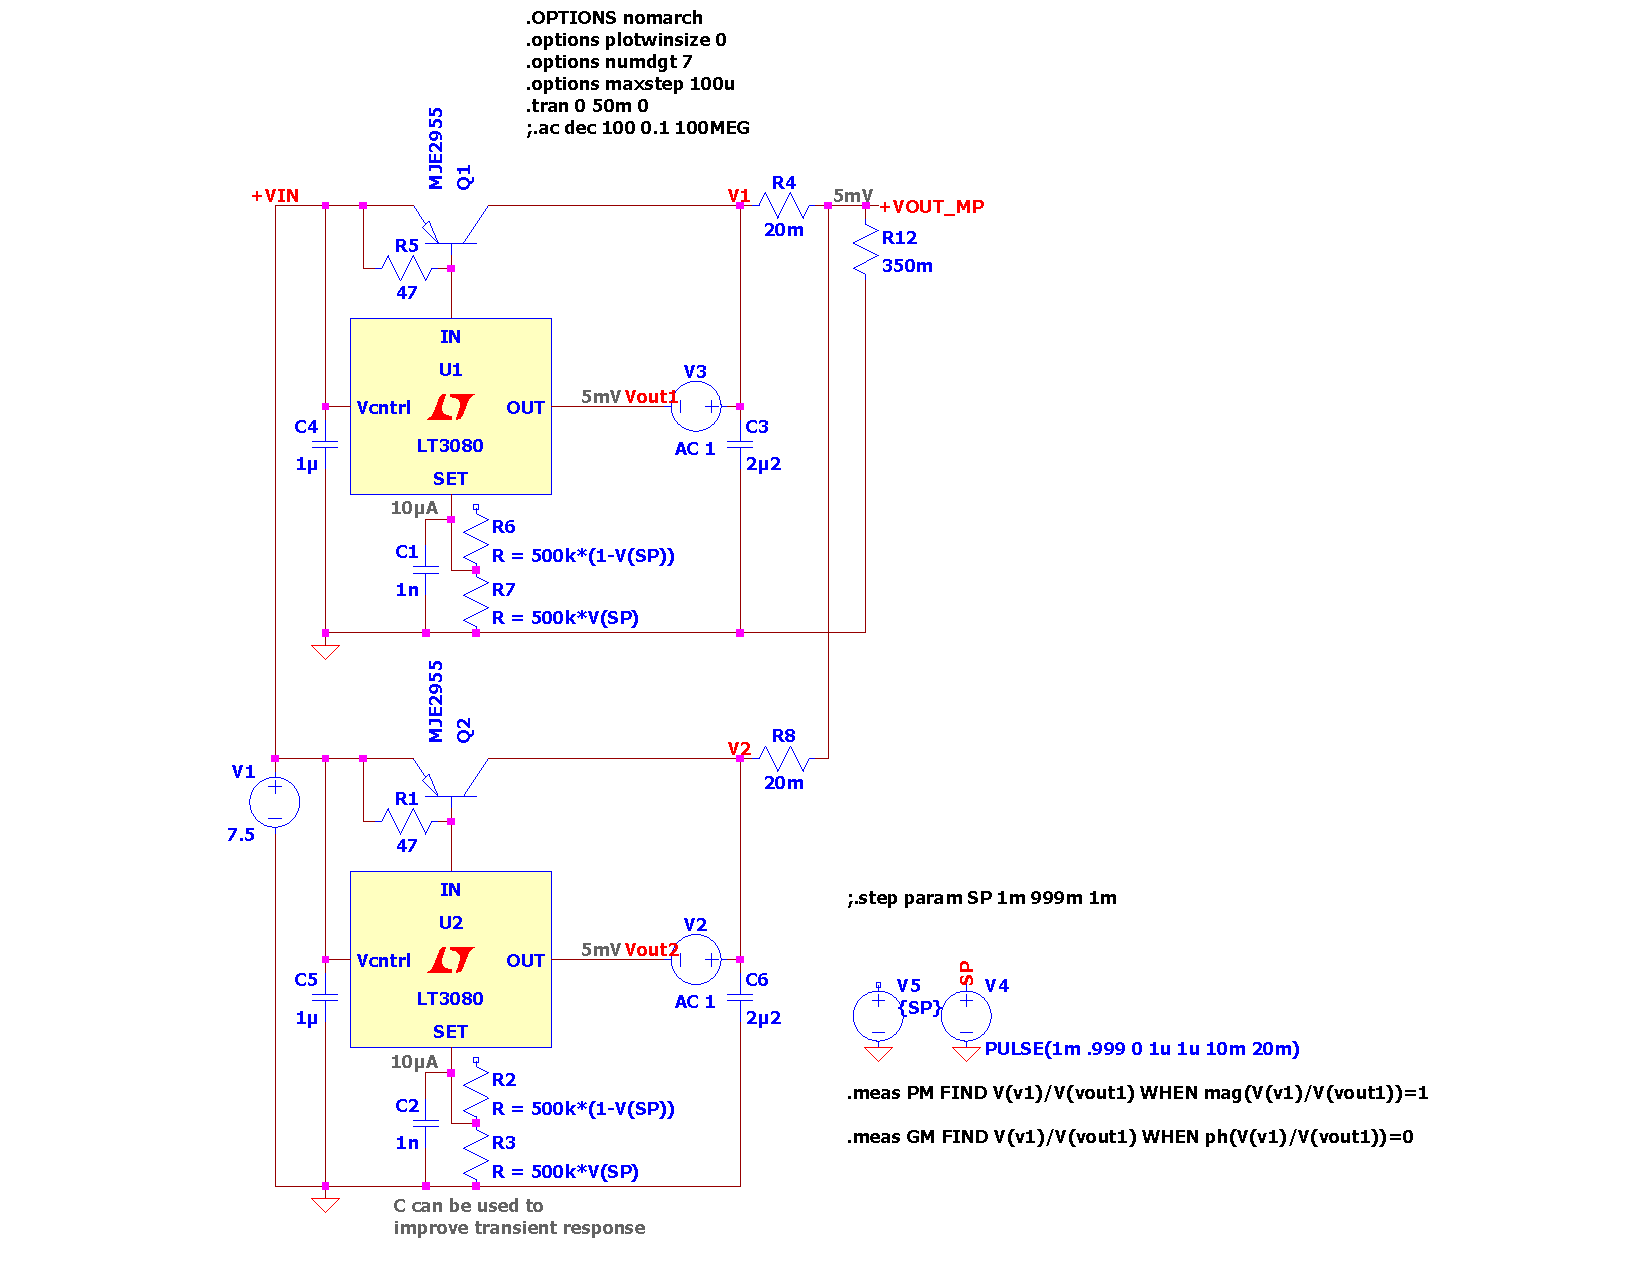
\includegraphics[width=0.45\textwidth]{LT3080-1_LinRegSchematic.pdf}
    \caption{12 A linear regulator design based on the LT3080-1.}
    \label{fig:LT3080-1_LinRegSchematic}
\end{figure}

The working of the circuit is as follows: the LT3080-1 is used as driver for the series pass PNP transistor which is used to amplify the current.
The output voltage can be set by changing the resistance between the set pin of the LT3080-1 and GND since the LT3080-1 incorporates a current source of 10 $\mu$A of which the high side is tied to the non-inverting input of an OpAmp. The output of this OpAmp is connected to its output pin via a NPN transistor and the emitter of this transistor is fed back to the inverting input of the OpAmp for feedback. Thus, the voltage on the output is forced to be the same as the voltage on its set pin, so according to Ohms law by changing the resistance between the set pin and GND the voltage across the resistor increases and so will the output voltage.

A 1 nF capacitor is placed at each set pin to GND to improve the transient response of the circuit by acting as a energy reservoir. Increasing its value further decreases the transient response since the used potentiometer in combination with this capacitor also forms a RC LPF. The series pass PNP transistor is biased with a 47 $\tcohm$ resistor to improve its GBW. The 1 $\mu$F input and 2.2 $\mu$F output capacitors are there for stability.

Two of these identical circuits are placed in parallel with their set pins tied together so they are at the same potential. To accommodate proper current sharing two 20 m$\tcohm$ series resistors have been added to give some feedback.
The transient response of the linear regulator is shown in Fig. \ref{fig:LT3080-1_LinRegSchematic} and shows that with an input voltage of 7.5 V an output voltage of 0 V up to around 6.9 V can be achieved. The phase margin over setpoint (current) is shown in Fig. \ref{fig:LT3080-1_Phase-margin_VS_setpoint}. The power dissipation in the main components is shown in Fig. \ref{fig:LT3080-1_PowerDissipation}.

\subsubsection{Sinking Current}
The current sink is based on an OpAmp driving a N-MOSFET in its linear region controlling the current flowing trough a sense resistor. The OpAmp changes its output so that the voltage across this sense resistor is equal to its setpoint derived from the digital potentiometer. The circuit is shown in \ref{fig:CurrentSinkSchematic} and the working of it is shown in Fig. \ref{fig:CurrentSinkTransient}. The resistor directly at the output of the OpAmp is there to limit the phase shift caused by the gate source capacitance of the MOSFET in combination with its parallel RC snubber. Together these components make the current sink stable in its intended operating region as shown in Fig. \ref{fig:CurrentSinkPM&GM}.

\begin{figure}[h!]
    \centering
    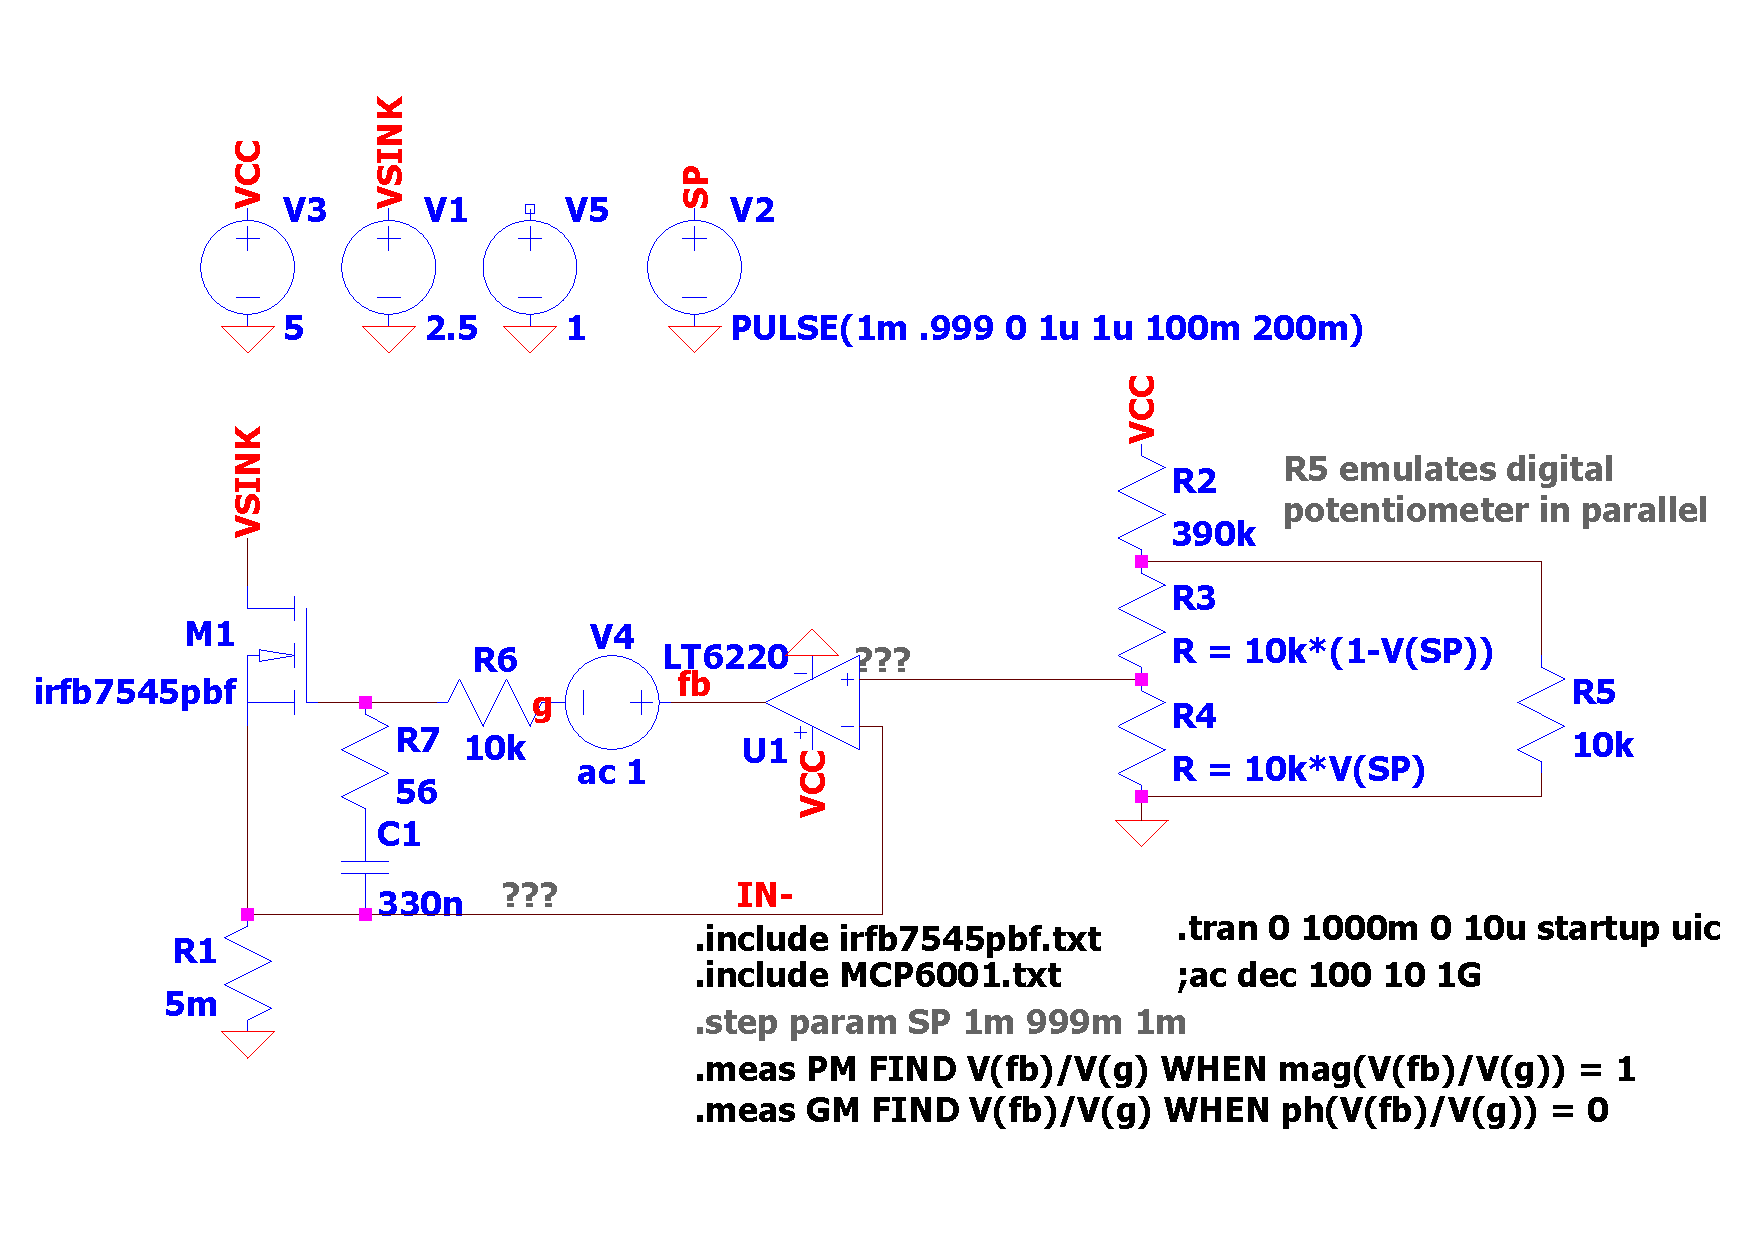
\includegraphics[width=0.45\textwidth]{CurrentSinkSchematic.pdf}
    \caption{12 A current sink schematic.}
    \label{fig:CurrentSinkSchematic}
\end{figure}

The corresponding KiCAD schematic is shown in Fig. \ref{fig:CellBoardKiCADSchematic}.

A model board has been made that interconnects all cell boards and incorporates a Atmega328PB MCU to control everything. The full schematic of this board is shown in Fig. \ref{fig:ModelBoardKiCADSchematic}. 

The mandatory reverse polarity protection on the model board is accomplished by adding a diode in series with the incoming supply rail.

\subsubsection{PCB design}
Since there are some substantial currents flowing through the design of up to 12 A the trace widths have been determined according to IPC2221A at a maximum temperature rise of 10 \textdegree C.

Since all cell boards must be able to be placed in series they should all be floating and be able to withstand at least the maximum expected cell voltage of each cell multiplied by the total amount of cells. Therefore, the minimum width of the isolation barrier has also been determined using IPC2221A.

\csvautotabular{TestPlan.csv}

\begin{table*}[!ht]
    \centering
    \begin{tabular}{|l|l|l|l|l|l|l|}
    \hline
        "ID" & Requirement & Test method & Expected outcome & Measured outcome & Check & Date \\ \hline
        1.1 & The maximum voltage of the 14 cell battery pack emulator is 80V & Attach Siglent SPD3303X-E power supply to input. Measure output voltage of the combined cells at maximum output voltage with a multimeter & 80V +- 10\% & ~ & ~ & ~ \\ \hline
        1.11 & The maximum voltage of the 4 cell battery pack emulator is 20V & Attach Siglent SPD3303X-E power supply to input. Measure output voltage of the combined cells at maximum output voltage with a multimeter & 20V +- 10\% & ~ & ~ & ~ \\ \hline
        1.2 & The battery pack emulator has a peak power of 13.44kW (see 10.1) & Attach Siglent SPD3303X-E power supply to input. Attach load to output and set output voltage of cell to maximum. Measure peak output voltage and current values with oscilloscope over time to calculate power.  & 13.44kW +- 10\% & ~ & ~ & ~ \\ \hline
        1.21 & The 4 cell battery pack emulator has a peak power of 240W (see 10.1) & Attach Siglent SPD3303X-E power supply to input. Attach load to output and set output voltage of cell to maximum. Measure peak output voltage and current values with oscilloscope over time to calculate power.  & 240W +- 10\% & ~ & ~ & ~ \\ \hline
        1.3 & The battery pack emulator has a continuous power of 112W (see 10.1) & Attach Siglent SPD3303X-E power supply to input. Attach load to output and set output voltage of cell to maximum. Measure output voltage and current with multimeter to calculate power.  & 112W +- 10\% & ~ & ~ & ~ \\ \hline
        5.1 & The emulated cell has a voltage range of 2.48 to 5.04 V & Attach Siglent SPD3303X-E power supply to input. Measure output voltage of each cell with multimeter at the minimum and maximum output voltages & 2.48V to 5.04V +-10\% & ~ & ~ & ~ \\ \hline
        5.2 & The emulated cell has a peak sourcing current of 12A & Attach Siglent SPD3303X-E power supply to input. Attach a load to the output and measure the current through the load & 12A +- 10\% & ~ & ~ & ~ \\ \hline
        5.3 & The emulated cell has a continuous sourcing current of 100mA & Attach Siglent SPD3303X-E power supply to input. Attach a load to the output and measure the current through the load & 100mA +- 10\% & ~ & ~ & ~ \\ \hline
        5.4 & The emulated cell has a peak sinking current of 12A & Take two Siglent SPD3303X-E power supplies in parallel and set the current to 6A and measure the current drawn from these supplies & 12A +- 10\% & ~ & ~ & ~ \\ \hline
        5.5 & The emulated cell has a continuous sinking current of 100mA & Take one Siglent SPD3303X-E power supply and set the current to 200mA and measure the current drawn from the supply & 100mA +- 10\% & ~ & ~ & ~ \\ \hline
        5.6 & The emulated cell has a peak power of 60W & Attach Siglent SPD3303X-E power supply to input. Attach load to output and set output voltage of cell to maximum. Measure peak output voltage and current values with oscilloscope over time to calculate power.  & 60W +- 10\% & ~ & ~ & ~ \\ \hline
        5.7 & The emulated cell has a continuous power of 0.5W & Attach Siglent SPD3303X-E power supply to input. Attach load to output and set output voltage of cell to maximum. Measure output voltage and current with multimeter to calculate power.  & 0.5W +- 10\% & ~ & ~ & ~ \\ \hline
        6.2 & A user interface is made to adjust the voltages & Set-up the user device and attach it to the PCB. Test for specific voltages, voltages on the boundaries, and if the voltages change in real time. Measure the output with a multimeter  & Output voltage responds to changes in the user interface & ~ & ~ & ~ \\ \hline
        6.3 & The voltages are adjusted using a digital potentiometer & Set-up the user device and attach it to the PCB. Vary the resistance of the potentiometer to achieve specific voltages and measure the output voltage of the PCB using a multimeter.   & Output voltage responds to changes in the digital potentiometer  & ~ & ~ & ~ \\ \hline
        7.1 & The temperature is emulated by using a digital potentiometer & Set-up the device and decide on reference temperatures. Set the digital potentiometer to the desired emulated temperature and measure.  & The emulated temperature matches the temperature from the potentiometer & ~ & ~ & ~ \\ \hline
        7.2 & The emulated temperature range is -40 to 80 C & Set-up the device. Set the digital potentiometer to emulate the desired temperature boundaries and measure.  & The emulated temperature range matches the desired range for the device  & ~ & ~ & ~ \\ \hline
        7.3 & The emulated battery pack has an output which indicates the temperature relative to the output voltage & ~ & ~ & ~ & ~ & ~ \\ \hline
        10.1 & The temperature of the electronics should be less than 25 C & *Run the device for an hour and then take the temperature of the electronics & Temperature is under 25 C & ~ & ~ & ~ \\ \hline
        10.2 & The input of the battery pack emulator has reverse polarity protection & Wire the input with inverse polarity  & nothing blows up & ~ & ~ & ~ \\ \hline
        10.3 & The input of the battery pack emulator and load emulator have over current protection & Increase the input current above the maximum value  & nothing blows up  & ~ & ~ & ~ \\ \hline
    \end{tabular}
\end{table*}